\documentclass[12pt]{article}
\usepackage[a4paper, total={6in, 8in}]{geometry}
\usepackage{amsfonts}
\usepackage{amsmath,amssymb,trimclip,adjustbox}
\usepackage{breqn}
\usepackage{hyperref}
\usepackage{tabularray}
\usepackage{flafter} 
\usepackage{polski}
\usepackage[utf8]{inputenc}

\setlength{\parindent}{0pt}
\setlength{\textheight}{720pt}
\setlength{\oddsidemargin}{0pt}
\setlength{\textwidth}{480pt}


\author{Michał Puchyr}
\title{Sprawozdanie z ćw 84 \\
WYZNACZANIE DŁUGOŚCI FALI ŚWIETLNEJ
ZA POMOCĄ SIATKI DYFRAKCYJNEJ}

\begin{document}
\maketitle

\section{Cel ćwiczenia}
\begin{itemize}
    \item Wyznaczenie długości fali emisji lasera lub innego źródła światła
    monochromatycznego
    \item Wyznaczenie stałej siatki dyfrakcyjnej
\end{itemize}

\section{Opis ćwiczenia}
\subsection{Wstęp teoretyczny}

\textbf{Siatka dyfrakcyjna} - przyrząd do przeprowadzania analizy widmowej światła. Tworzy ją układ równych, równoległych i jednakowo rozmieszczonych szczelin.

\textbf{Stała siatki dyfrakcyjnej} to parametr charakteryzujący siatkę dyfrakcyjną. Wyraża on rozstaw szczelin siatki (odległość między środkami kolejnych szczelin).

Działanie siatki dyfrakcyjnej polega na wykorzystaniu zjawiska dyfrakcji i interferencji światła do uzyskania jego widma. 
W tym celu pomiędzy źródłem światła a ekranem umieszcza się siatkę dyfrakcyjną. 
Na ekranie uzyskuje się w ten sposób widmo światła. \\

Przyrządy i materiały wykorzystane do pomiarów : 

\begin{itemize}
    \item Transmisyjne siatki dyfrakcyjne (S) : typ „A” -50 linii na milimetr oraz typ „B”
    \item Laser emitujący zielone światło (PM)
    \item Ekran ze skalą milimetrową (E)
    \item Ława optyczna ze skalą milimetrową
    \item Szczelina (O)
\end{itemize}

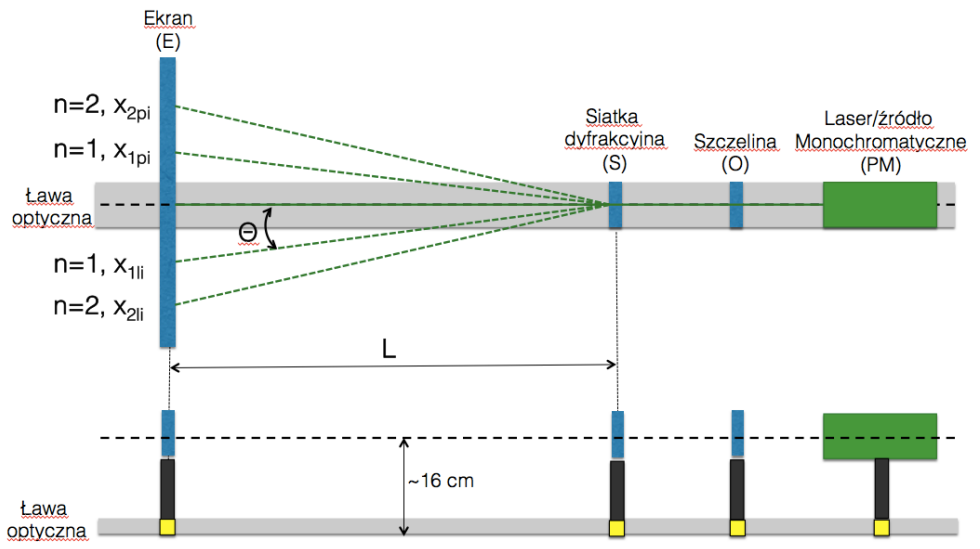
\includegraphics[scale = 0.63]{schemat.png} \\
Schemat układu eksperymentalnego

\section{Pomiary układu}

\begin{table}[!htbp]
    \centering
    \begin{adjustbox}{width=1\textwidth}
    \begin{tabular}{|c|c|c|c|c|c|c|}
    \hline
    \multicolumn{7}{|c|}{Wyniki pomiarów dla wyznaczenia dł. fali linii monochromatycznej źródła} \\
    \hline
        L$_i$(mm) & u(L$_i$)(mm) & n & x$_{lni}$(mm) & u(x$_{lni}$)(mm) & x$_{lpi}$(mm) & u(x$_{lpi}$)(mm) \\ \hline
        300 & 0,58 & 1 & 8 & 2 & 8 & 2 \\
        ~ & 0,58 & 2 & 17 & 2 & 17 & 2 \\ 
        ~ & 0,58 & 3 & 24 & 2 & 24 & 2 \\ \hline
        350 & 0,58 & 1 & 9 & 2 & 9 & 2 \\
        ~ & 0,58 & 2 & 19 & 2 & 19 & 2 \\ 
        ~ & 0,58 & 3 & 28 & 2 & 28 & 2 \\ \hline
        400 & 0,58 & 1 & 11 & 2 & 11 & 2 \\ 
        ~ & 0,58 & 2 & 22 & 2 & 22 & 2 \\ 
        ~ & 0,58 & 3 & 33 & 2 & 32 & 2 \\ \hline
        450 & 0,58 & 1 & 13 & 2 & 13 & 2 \\ 
        ~ & 0,58 & 2 & 24 & 2 & 24 & 2 \\ 
        ~ & 0,58 & 3 & 37 & 2 & 37 & 2 \\ \hline
        500 & 0,58 & 1 & 14 & 2 & 14 & 2 \\ 
        ~ & 0,58 & 2 & 27 & 2 & 26 & 2 \\ 
        ~ & 0,58 & 3 & 40 & 2 & 40 & 2 \\ \hline
    \end{tabular}
\end{adjustbox}
\end{table}

\begin{table}[!htbp]
    \centering
    \begin{adjustbox}{width=1\textwidth}
    \begin{tabular}{|c|c|c|c|c|c|}
    \hline
    \multicolumn{6}{|c|}{Wyniki pomiarów dla wyznaczenia stałej siatki dyfrakcyjnej} \\
    \hline
        L$_i$(mm) & u(L$_i$)(mm) & x$_{li}$(mm) & u(x$_{li}$)(mm) & x$_{pi}$(mm) & u(x$_{pi}$)(mm) \\ \hline
        50 & 0,58 & 32 & 2 & 32 & 2 \\ \hline
        80 & 0,58 & 49 & 2 & 49 & 2 \\ \hline
        110 & 0,58 & 69 & 2 & 69 & 2 \\ \hline
        140 & 0,58 & 87 & 2 & 87 & 2 \\ \hline
        170 & 0,58 & 105 & 2 & 106 & 2 \\ \hline
        200 & 0,58 & 125 & 2 & 125 & 2 \\ \hline
        230 & 0,58 & 143 & 2 & 144 & 2 \\ \hline
        260 & 0,58 & 162 & 2 & 162 & 2 \\ \hline
        290 & 0,58 & 181 & 2 & 181 & 2 \\ \hline
        320 & 0,58 & 200 & 2 & 200 & 2 \\ \hline
        350 & 0,58 & 218 & 2 & 217 & 2 \\ \hline
        380 & 0,58 & 237 & 2 & 238 & 2 \\ \hline
        410 & 0,58 & 255 & 2 & 255 & 2 \\ \hline
        440 & 0,58 & 275 & 2 & 275 & 2 \\ \hline
        470 & 0,58 & 295 & 2 & 295 & 2 \\ \hline
    \end{tabular}
\end{adjustbox}
\end{table}

\begin{table}[!htbp]
    \centering
\begin{adjustbox}{width=1\textwidth}
    \begin{tabular}{|c|c|c|c|c|c|c|}
    \hline
    \multicolumn{7}{|c|}{Wyniki obliczeń dla wyznaczenia dł. fali linii monochromatycznej źródła} \\
    \hline
        L$_{n,i}$(mm) & u(L$_{n,i}$)(mm) & $\overline{x}_{n,i}$ & u($\overline{x}_{n,i}$)(mm) & $\sin \Theta$ & u($\sin \Theta$) & $\lambda(nm)$ \\ \hline
        300 & 0,58 & 8 & 2 & 0,027 & 0,007 & 540,00 \\ \hline
        300 & 0,58 & 17 & 2 & 0,057 & 0,007 & 570,00 \\ \hline
        300 & 0,58 & 24 & 2 & 0,080 & 0,007 & 533,34 \\ \hline
        350 & 0,58 & 9 & 2 & 0,026 & 0,006 & 520,00 \\ \hline
        350 & 0,58 & 19 & 2 & 0,055 & 0,006 & 550,00 \\ \hline
        350 & 0,58 & 28 & 2 & 0,080 & 0,006 & 533,34 \\ \hline
        400 & 0,58 & 11 & 2 & 0,028 & 0,005 & 560,00 \\ \hline
        400 & 0,58 & 22 & 2 & 0,055 & 0,005 & 550,00 \\ \hline
        400 & 0,58 & 33 & 2 & 0,081 & 0,005 & 540,00 \\ \hline
        450 & 0,58 & 13 & 2 & 0,029 & 0,005 & 580,00 \\ \hline
        450 & 0,58 & 24 & 2 & 0,054 & 0,005 & 540,00 \\ \hline
        450 & 0,58 & 37 & 2 & 0,082 & 0,005 & 546,67 \\ \hline
        500 & 0,58 & 14 & 2 & 0,028 & 0,004 & 560,00 \\ \hline
        500 & 0,58 & 27 & 2 & 0,053 & 0,004 & 530,00 \\ \hline
        500 & 0,58 & 40 & 2 & 0,080 & 0,004 & 533,34 \\ \hline
        \multicolumn{6}{|l|}{Wartość średnia: $\overline{\lambda}(nm)=$} & 545,78 \\ \hline
        \multicolumn{6}{|l|}{Odchylenie standardowe: $u(\overline{\lambda})(nm)=$} & 4,19 \\ \hline
    \end{tabular}
\end{adjustbox}
\end{table}

\begin{table}[!htbp]
    \centering
    \begin{adjustbox}{width=1\textwidth}
    \begin{tabular}{|c|c|c|c|c|}
    \hline
    \multicolumn{5}{|c|}{Wyniki obliczeń dla wyznaczenia stałej siatki dyfrakcyjnej} \\
    \hline
        L$_i$(mm) & $\overline{x}_i$(mm) & u($\overline{x}_i$)(mm) & $\sin \Theta$ & u$_c(\sin \Theta)$ \\ \hline
        50 & 32 & 2 & 0,540 & 0,025 \\ \hline
        80 & 49 & 2 & 0,523 & 0,016 \\ \hline
        110 & 69 & 2 & 0,532 & 0,012 \\ \hline
        140 & 87 & 2 & 0,528 & 0,009 \\ \hline
        170 & 106 & 2 & 0,530 & 0,008 \\ \hline
        200 & 125 & 2 & 0,530 & 0,007 \\ \hline
        230 & 144 & 2 & 0,531 & 0,006 \\ \hline
        260 & 162 & 2 & 0,529 & 0,005 \\ \hline
        290 & 181 & 2 & 0,530 & 0,005 \\ \hline
        320 & 200 & 2 & 0,530 & 0,004 \\ \hline
        350 & 218 & 2 & 0,529 & 0,004 \\ \hline
        380 & 238 & 2 & 0,531 & 0,004 \\ \hline
        410 & 255 & 2 & 0,529 & 0,004 \\ \hline
        440 & 275 & 2 & 0,530 & 0,003 \\ \hline
        470 & 295 & 2 & 0,532 & 0,003 \\ \hline
    \multicolumn{4}{|l|}{Wartość średnia : $\overline{\sin \Theta}=$} & 0,531 \\ \hline
    \multicolumn{4}{|l|}{Odchylenie standardowe : u($\overline{\sin \Theta})=$} & 0,0009 \\ \hline
    \multicolumn{4}{|l|}{$d(nm)$} & 1029,78 \\ \hline
    \multicolumn{4}{|l|}{$u_c(d)(nm)=$} & 8,08 \\ \hline
    \end{tabular}
\end{adjustbox}
\end{table}


\section{Przykładowe obliczenia}

\subsection{Obliczenia dla pierwszej części eksperymentu}

Obliczenie średniej wartości odległości linii dyfrakcyjnej od pozycji
zerowego rzędu dyfrakcji : 

$$ \overline{x}_{n,i} = \frac{x_{nli} + x_{npi}}{2} = \frac{17 + 17}{2} = 17[mm]$$

$$ u(\overline{x}_{n,i}) = \frac{u(x_{nli}) + u(x_{npi})}{2} = \frac{2 + 2}{2} = 2[mm] $$ \\

Obliczenie sinusa kąta ugięcia :

$$ \sin \Theta_{n,i} = \frac{\overline{x}_{n,i}}{\sqrt{\overline{x}^{2}_{n,i} + L^{2}_i}}
= \frac{8}{\sqrt{8^2 + 300^2}} = 0.02665 \approx 0,027 $$

$$ u_c(\sin \Theta_{n,i}) = \sqrt{\left(\frac{L_i \overline{x}_{n,i}}{\left(L^2_i + \overline{x}^2_{n,i}\right)^{\frac{3}{2}}}\right)^2 u^2(L) + 
\left(\frac{L^2_i}{(L^2_i + \overline{x}^2_{n,i})^{\frac{3}{2}}}\right)^2 u^2(\overline{x}_{n,i})} = $$

$$ = \sqrt{\left( \frac{300 \cdot 8}{\left(300^2 + 8^2\right)^{\frac{3}{2}}} \right)^2 \cdot (0,58)^2 +
\left( \frac{300^2}{\left(300^2 + 8^2 \right)^{\frac{3}{2}}} \right)^2 \cdot 2^2 } = 0,00665 \approx 0,007 $$\\

Długość fali emisji światła emitowanego przez laser :

$$ \lambda_{n,i} = \frac{d \cdot (\sin \Theta_{n,i})}{n} = \frac{\frac{1}{50} \cdot 0,007}{1}
= 0,00054[mm] \approx 540[nm] $$

$$ \overline{\lambda}_{n,i} = \frac{\sum\limits_{i = 1}^{n} \lambda_{i}}{n} =
\frac{540,00 + 570,00 + ... + 530,00 + 533,34}{15} = \frac{8186,69}{15} = 545,7793 \approx 545,78[nm] $$ \\

$$ u(\overline{\lambda}) = \sqrt{ \frac{\sum\limits_{i = 1}^{n} \left(\lambda_i - \overline{\lambda} \right)^2}{n(n-1)} }
= \sqrt{ \frac{33,40 + 586,64 + ... + 248,98 + 154,737}{15 \cdot 14} } $$
$$= \sqrt{\frac{3676,545}{210}} = 4,18418 \approx 4,19 $$

\pagebreak

\subsection{Obliczenia dla drugiej części eksperymentu}

Obliczenia dla pierwszych trzech danych są identyczne jak w pierwszej części eksperymentu. \\

Obliczenie średniej $ \overline{\sin \Theta}$

$$ \overline{\sin \Theta} = \frac{\sum\limits_{i = 1}^{n} \sin \Theta_i}{n} = 
\frac{0,540 + 0,523 + ... + 0,530 + 0,532}{15} = \frac{7,954}{15} = 0,53026 \approx 0,531 $$ \\

Obliczenie odchylenia standardowego $u(\overline{\sin \Theta})$

$$ u(\overline{\sin \Theta}) = \sqrt{ \frac{\sum\limits_{i = 1}^{n} \left(\sin \Theta_i - \overline{\sin \Theta} \right)^2}{n(n-1)} } 
= \sqrt{ \frac{0,000166}{210} } = 0,00088908 \approx 0,0009 $$ \\

Obliczenie stałej siatki dyfrakcyjnej d (dla widma n = 1):

$$ d = \frac{n \overline{\lambda}}{\overline{\sin \Theta}} = \frac{1 \cdot 545,78}{0,53} = 1029,774 \approx 1029,78[nm] $$

Obliczenie wartości niepewności związanej z wyznaczeniem stałej siatki dyfrakcyjnej \linebreak (dla widma n = 1):

$$ u_c(d) = \sqrt{ \left( \frac{n}{\overline{\sin \Theta}} \right)^2 u^2(\overline{\lambda}) +
\left( \frac{n \overline{\lambda}}{\overline{\sin \Theta}^2} \right)^2 u^2(\overline{\sin \Theta}) } = 
\sqrt{ \left( \frac{1}{0,531} \right)^2 \cdot 4,19^2 + \left( \frac{1 \cdot 545,78}{0,531^2} \right)^2 \cdot 0,0009^2 } $$
$$ = \sqrt{62,26428 + 3,03488} = \sqrt{65,29916} = 8,08079 \approx 8,08[nm] $$

\section{Wnioski}

Przy pomocy pomiarów odczytanych z ekranu udało się wyznaczyć długość fali lasera. Jest ona zgodna
z teoretycznymi przewidywaniami, zakres długości fali świetlnej dla zielonej barwy mieści się w przedziale
od około 520 nm do 565 nm. Zmierzona średnia długość fali świetlnej w eksperymencie wynosi 545,78
$ \pm \ 4,19 $ nm co 
potwierdza poprawność przeprowadzonych pomiarów.

W drugiej części eksperymentu wyznaczona została stała siatki dyfrakcyjnej B, która według pomiarów 
wynosi 1029,78 $ \pm \ 8,08 $ nm co daje nam około 972 $ \frac{rys}{mm}. $

\section{Bibliografia}
\begin{itemize}
    \item \url{https://pl.wikipedia.org/wiki/Barwy_proste}
    \item \url{https://pl.wikipedia.org/wiki/Siatka_dyfrakcyjna}
\end{itemize}

\end{document}